\documentclass[10pt,letterpaper]{article}
\usepackage[utf8]{inputenc}
\usepackage[english]{babel}
\usepackage{amsmath}
\usepackage{amsfonts}
\usepackage{amssymb}
\usepackage{makeidx}
\usepackage{graphicx}
\usepackage{lmodern}
\usepackage{kpfonts}
\usepackage{multirow}

\usepackage{listings}
\usepackage{xcolor}
\definecolor{codegreen}{rgb}{0,0.6,0}
\definecolor{codegray}{rgb}{0.5,0.5,0.5}
\definecolor{codepurple}{rgb}{0.58,0,0.82}
\definecolor{backcolour}{rgb}{0.95,0.95,0.92}
\lstdefinestyle{mystyle}{
    backgroundcolor=\color{backcolour},   
    commentstyle=\color{codegreen},
    keywordstyle=\color{magenta},
    numberstyle=\tiny\color{codegray},
    stringstyle=\color{codepurple},
    basicstyle=\ttfamily\footnotesize,
    breakatwhitespace=false,         
    breaklines=true,                 
    captionpos=b,                    
    keepspaces=true,                 
    numbers=left,                    
    numbersep=5pt,                  
    showspaces=false,                
    showstringspaces=false,
    showtabs=false,                  
    tabsize=2
}
\lstset{style=mystyle}

\usepackage[left=2cm,right=2cm,top=2cm,bottom=2cm]{geometry}
\title{Big O Notation}
\author{Elshad Karimov}
\begin{document}
\begin{titlepage}
\maketitle
\end{titlepage}
\section{Analogy and Time Complexity}
Big O is the language and metric we use to describe the efficiency of algorithms.\\

\textbf{Type}:
$O(N)$, $O(n^{2})$ and $o(2^{N})$.

\section{Big O, Big $\Theta$ and Big $\Omega$}
Algorithm run time notations. Just as the car performance evaluation.
\begin{itemize}
\item City traffic -20 liters / 100 km. (Worse case)
\item Highway - 10 liters / 100 km. (Best case)
\item Mixed condition - 15liters / 100 km. (Average case)
\end{itemize}
\textbf{Big O, Big $\Theta$ and Big $\Omega$}
\begin{itemize}
\item \textbf{Big O}: It is a complexity that is going to be less or equal to the worst case.
\item \textbf{Big $\Omega$}: It is a complexity that is going to be at least more than the best case.
\item \textbf{Big $\Theta$}: It is a complexity that is within bounds of the worst and the best case.
\end{itemize}

\begin{figure}[hbtp]
\caption{Number Finding Algorithm}
\centering
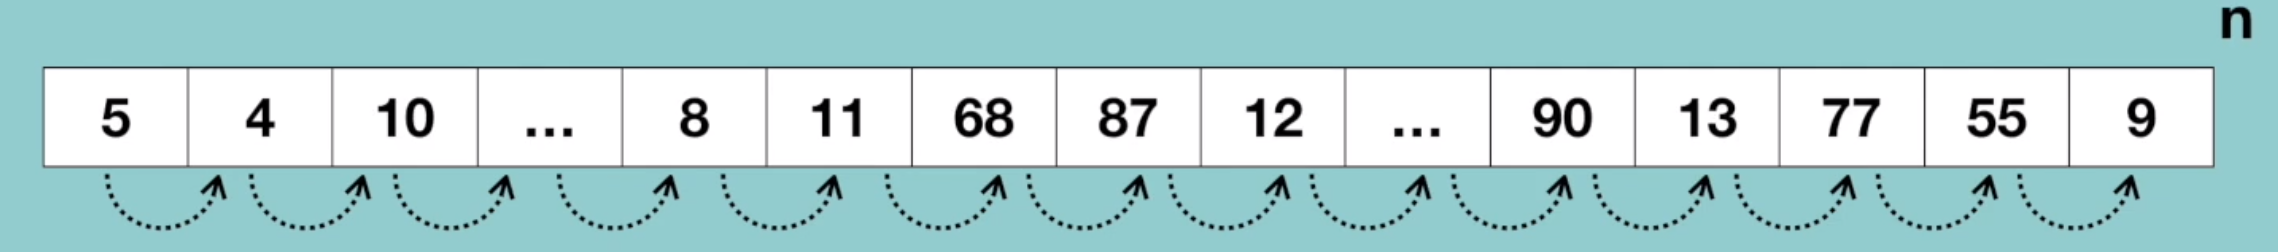
\includegraphics[scale=0.2]{images/Screenshot from 2021-06-30 20-24-08.png}
\end{figure}

\begin{itemize}
\item \textbf{Big $O$ - $O(N)$}
\item \textbf{Big $\Omega$ - $\Omega(1)$}
\item \textbf{Big $\theta$ - $\theta(n/2)$}
\end{itemize}

\section{Algorithm Time Complexity Examples}

\begin{table}[hbtp]
\caption{Algorithm run time complexities}
\centering
\begin{tabular}{|l|l|l|}
\hline
\textbf{Complexity}&\textbf{Name}&\textbf{Sample}\\
\hline
$O(1)$ & Constant & Accessing a specific element in array \\
\hline
$O(N)$ & Linear & Loop through array elements \\
\hline
$O(LogN)$ & Logarithmic & Find an element in sorted array \\
\hline
$O(N^{2})$ & Quadratic & Looking ar a every index in the array twice \\
\hline
$O(2^{N}$ & Exponential & Double recursion in Fibonacci\\
\hline
\end{tabular}
\end{table}

\textbf{$O(1)$-Constant time}
\begin{lstlisting}[language=Python]
# It takes constant time to access first element
array = [1,2,3,4,5]
array[0] 
\end{lstlisting}

\textbf{$O(N)$-Linear time}
\begin{lstlisting}[language=Python]
# Linear time since it is visiting every element of array
array = [1,2,3,4,5]
for element in array:
	print(element)
\end{lstlisting}

\textbf{$O(logN)$-Logarithmic time}
\begin{lstlisting}[language=Python]
# Logarithmic time since it is visiting only some elements
for index in range(0, len(array),3):
	print(array[index])
\end{lstlisting}
\begin{lstlisting}[language=Python]
# Binary search
search 9 within [1,5,8,9,11,13,15,19,21]
compare 9 to 11 then smaller
search 9 within [1,5,8,9]
compare 9 to 8 then bigger
search 9 within [9]
compare 9 to 9
return 
\end{lstlisting}

\textbf{$O(N^{2})$-Quadratic time}
\begin{lstlisting}[language=Python]
array = [1,2,3,45]
for x in array:
	for y in array:
		print(x,y)
\end{lstlisting}

\textbf{$O(2^{N})$-Exponential time}
\begin{lstlisting}[language=Python]
def fibonacci(n)
	if n <= 1:
		return n
	return fibonacci(n-1)+fibonacci(n-2)
\end{lstlisting}

\begin{figure}[hbtp]
\centering
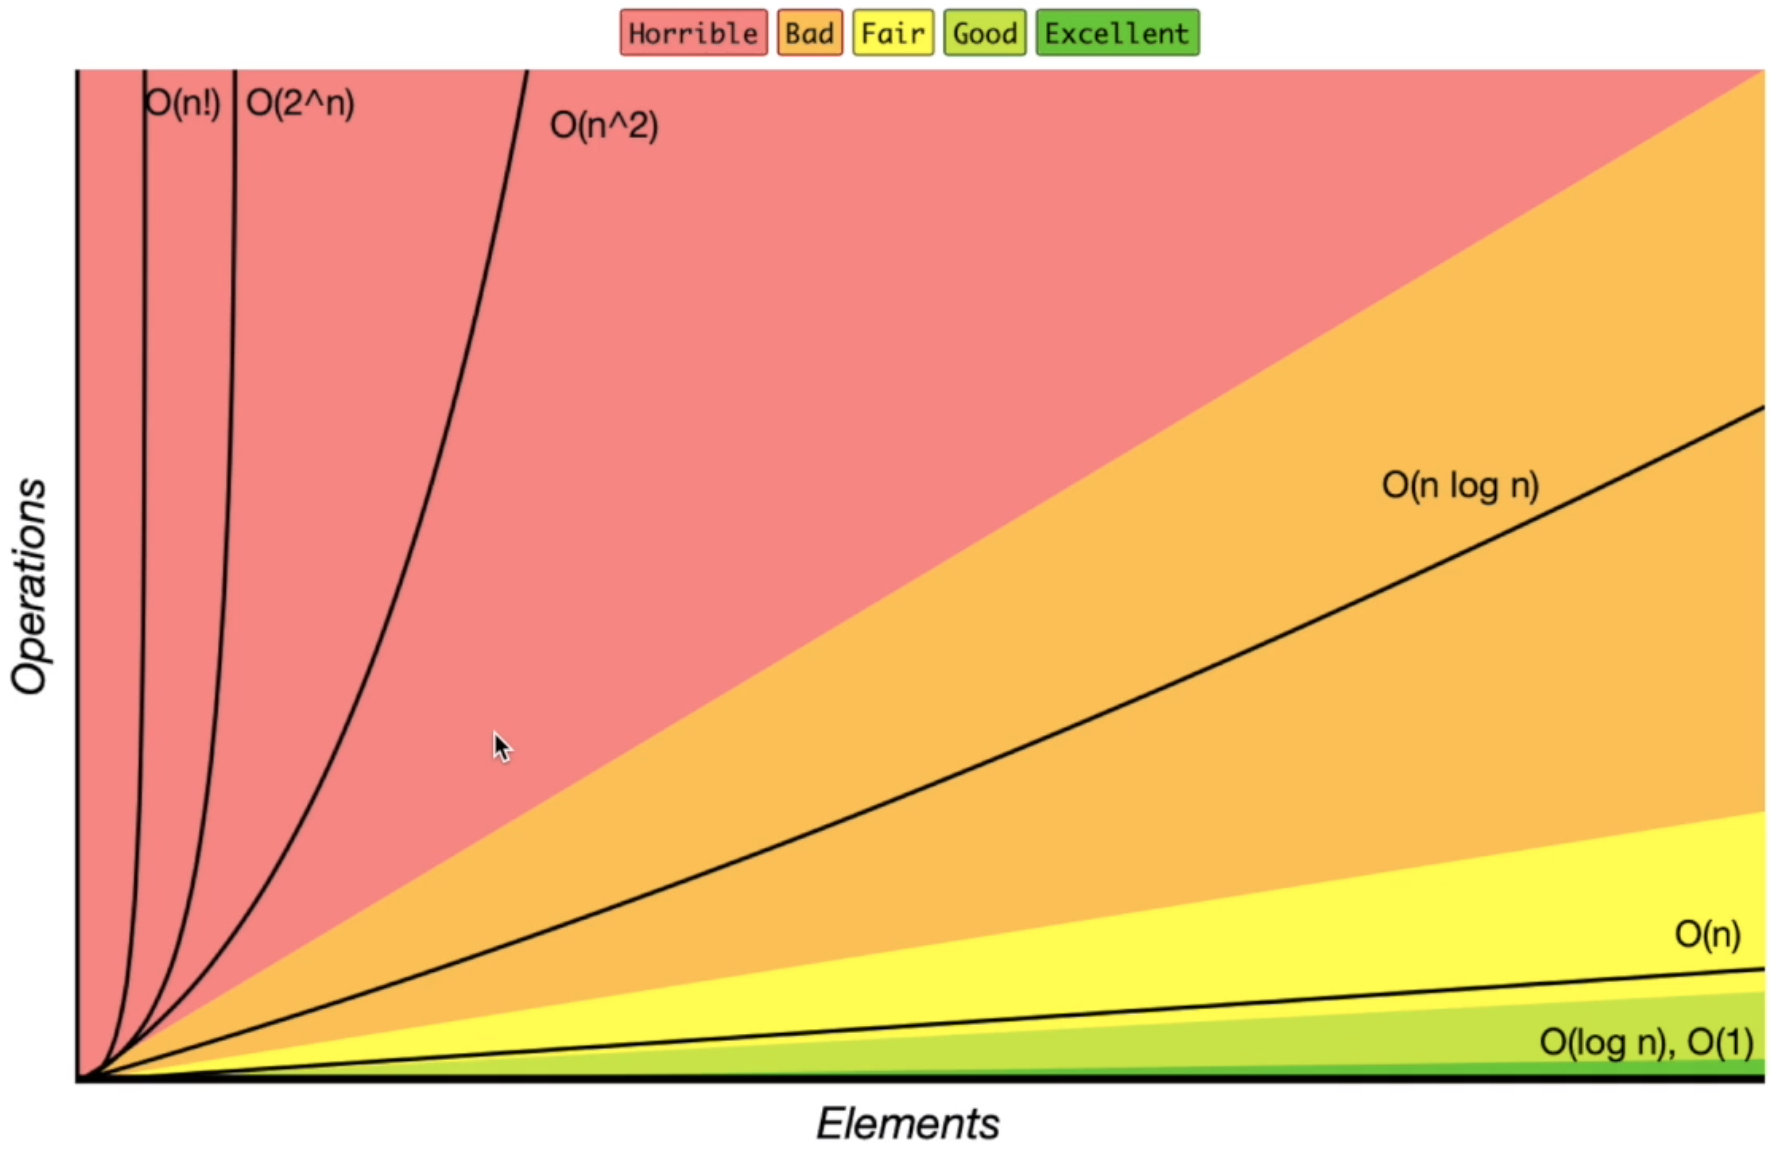
\includegraphics[scale=0.2]{images/Screenshot from 2021-07-01 01-23-01.png}
\caption{Big-O Complexity Chart}
\end{figure}

\section{Space Complexity}


































\end{document}